\section{Scanning}
\label{sec:scanning}

Zusätzlich zur Netzmessung wurde die Schwergewichtsmauer im Bereich 'Sperre'~\ref{fig:abb-schwergewmauer} 
mittels terrestrischem Laserscanning (TLS) flächenhaft erfasst. Die Aufnahmen erfolgten von fünf Stationen 
mittels einer Trimble SX12. Daraus resultieren direkt georeferenzierte Punktwolken.

\begin{figure}[h!]
    \centering
    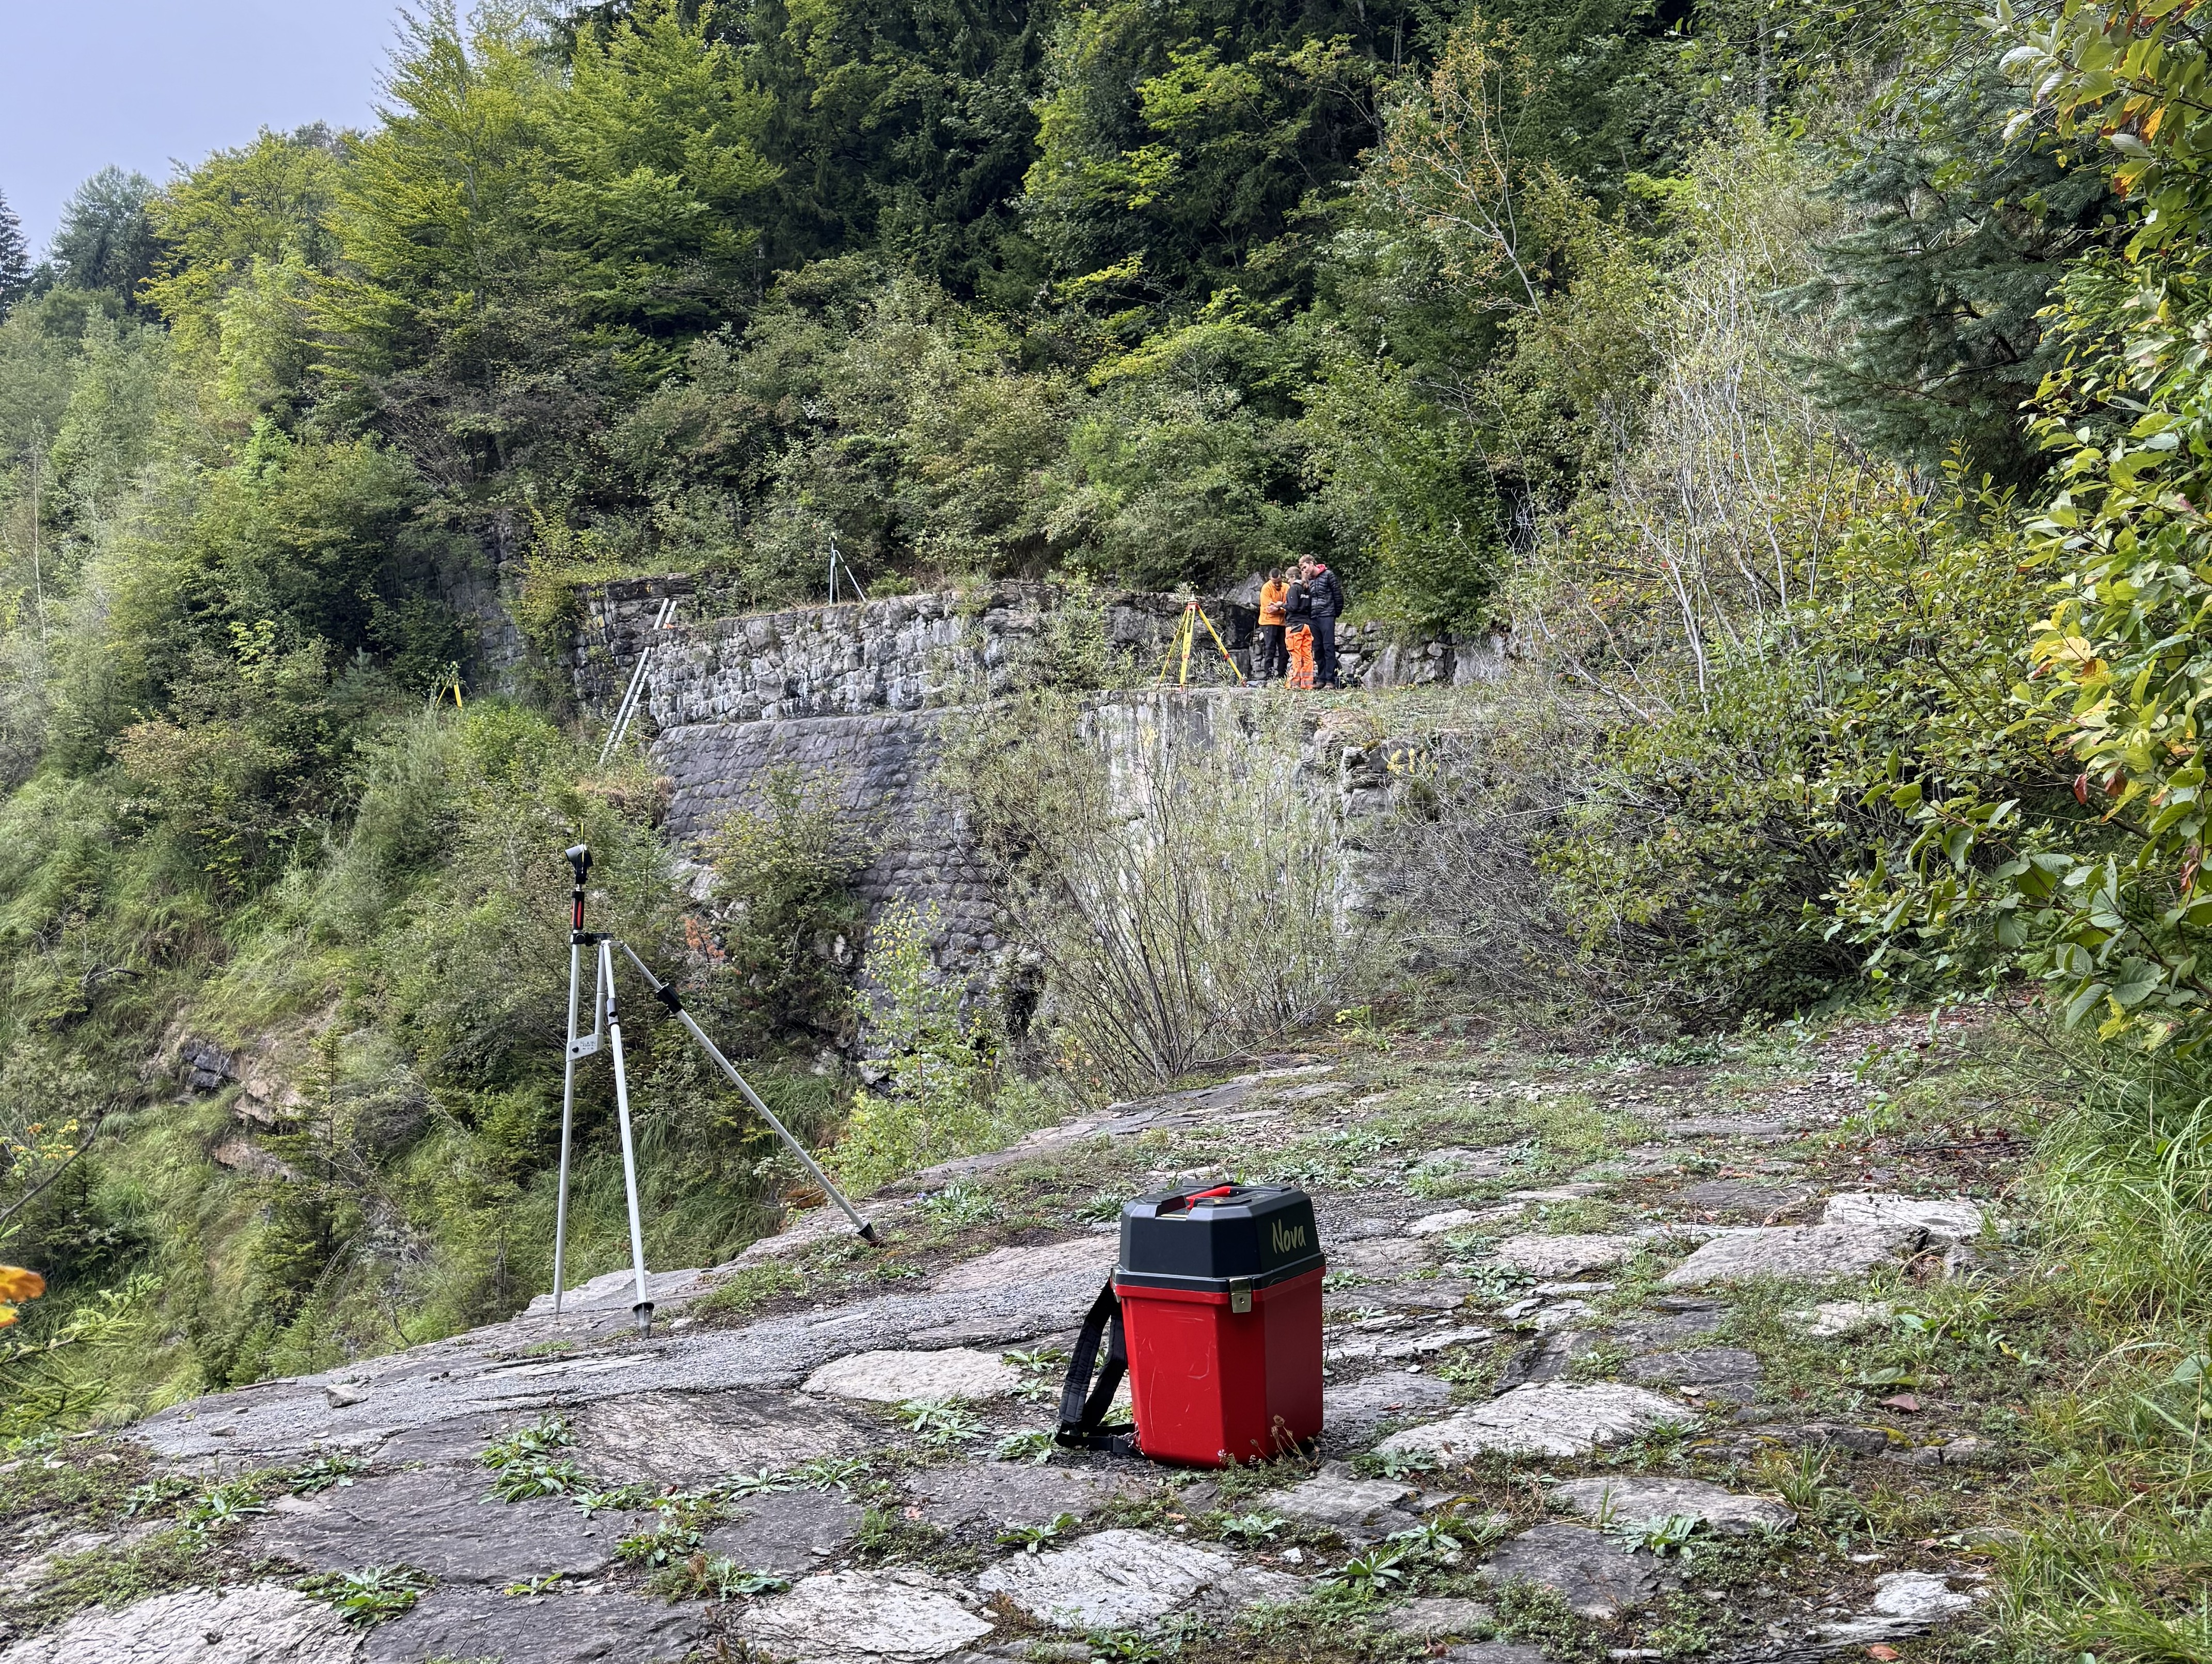
\includegraphics[width=\textwidth]{Schwergewichtsmauer.jpg}
    \caption{Aufnahme Schwergewichtsmauer und Netzmessung im Feldkurs 2026}
    \label{fig:abb-schwergewmauer}
\end{figure}

\subsection{Datenaufbereitung und Auswertung}
\label{sec:datenaufbereitung}

Die Scanstationen werden im Trimble Business Center (TBC) \parencite{noch zitieren TBC} anhand der ausgeglichenen Koordinaten der Netzmessung neu registriert. 
Dadurch sinkt die Standardabweichung der Lage und Höhe der einzelnen Stationierungen auf $\sigma < 1 mm$.
Danach wird in Trimble RealWorks \parencite{noch zitieren TRW} die Punktwolke bereinigt und so zugeschnitten, dass sie mit der Aufnahme von letzter
Epoche verglichen werden kann. Die automatische Klassifikation zur Bereinigung ist hier jedoch nicht immer sehr hilfreich,
da die Mauern 'schräger' sind als normale Mauern oder Wände und somit nicht als diese erkannt werden.
Somit folgt eine längere manuelle Bereinigung von Vegetation und Fremdobjekten.

Der Vergleich der beiden Punktwolken findet in CloudCompare \parencite{noch zitieren CC} statt.

% pro wolke je 3mm registrierungsgenauigketi
% m3c2 algorithmus -> vergleich
% distanzungenauigkeit

% selbes problem aus unserem paper sichtbar:
% "fassadenseite" weist sichtbare differenzen von bis zu 10 cm aus, obendrauf ist kaum eine verschiebung erkennbar
% liegt daran, dass m3c2 algorithmus nur verschiebungen zur fläche und nicht parallel dazu erkennen kann

\subsection{Resultate}
\label{sec:resultate}

\subsection{Diskussion der Resultate}
\label{sec:diskussion der resultate}